\documentclass{article}
\usepackage{standalone}
\usepackage{tikz}
\usetikzlibrary{calc,arrows}
\begin{document}

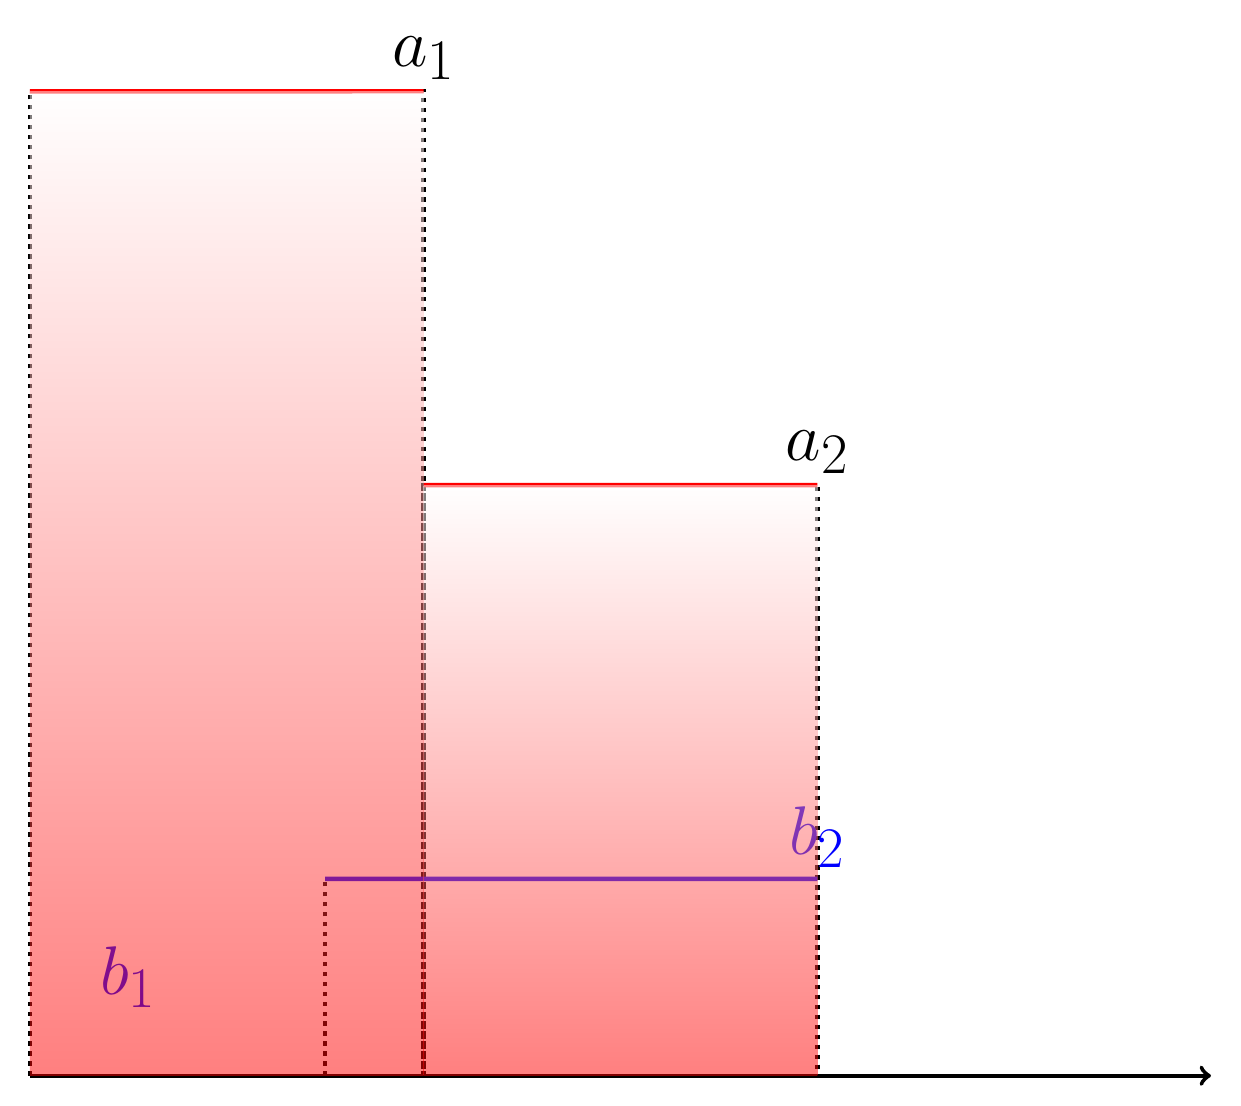
\begin{tikzpicture}[scale=2.5]
    % Important coordinates are defined
    \coordinate (beg_1) at (2,5);
    \coordinate (beg_2) at (2,0);
    \coordinate (end_2) at (4,3);
    \coordinate (end_3) at  (4,1);
    %\coordinate (beg_2) at ($(beg_1)+(1,0)$);
    %\coordinate (dev_1) at ($(beg_2)+(0,-.75)$);
    %\coordinate (xint) at (3,0);
    %\coordinate (end) at (5,1.25);

    \draw[ultra thick,->] (0,0) -- (6,0);
    \draw[ultra thick,dotted] (0,0) rectangle (beg_1) node[above] {\Huge$a_1$};
    \draw[ultra thick,dotted] (beg_2) rectangle (end_2) node[above] {\Huge$a_2$};
    \draw[ultra thick,blue] (1.5,1) -- (end_3) node [above] {\Huge{$b_2$}};
    \draw[ultra thick,dotted] (1.5,0) -- (1.5,1);
    \draw[ultra thick,red] (0,5) -- (beg_1);
    \draw[ultra thick,red] (2,3) -- (end_2);
    \node[blue] at (0.5,0.5) {\Huge$b_1$};
    \begin{scope}[opacity=0.5]
        \shade[top color=white, bottom color=red]
            (0,0) rectangle (beg_1);
    \end{scope}
    \begin{scope}
        \shade[top color=white, bottom color=red][opacity = 0.5]
            (beg_2) rectangle (end_2);
    \end{scope}
\end{tikzpicture}
\end{document}
